There are two main approaches to develop specialized propagation algorithms for global constraints:
\begin{itemize}
    \renewcommand{\labelitemi}{}
    \item $1^{st}$ \textbf{Constraint decomposition}. \\
    The main idea about constraint decomposition is to divide a \textbf{global constraint} into smaller and simpler constraints, each of which has a 
    known propagation algorithm. So basically we express a global constraint as a conjuction of smaller constraints propagation algorithms.
    \begin{example}
        e.g. Let's take a look again at the $\textit{among}(\dots)$ counting constraint. 
        $$ 
            \begin{gathered}
                \textit{among}([X_1, \dots, X_k], s, N) \text{ holds if and only if } \\
                N = |\{i | X_i \in s, 1 \leq i \leq k \}|
            \end{gathered}
        $$
        Assuming that our solver does not have the $\textit{among}(\dots)$ constraint resolution, it is just a decomposition as a conjuction of logical
        constraints and a sum constraint:
        \begin{enumerate}
            \item $B_i$ with $D(B_i) = \{0, 1\}$ for $1 \leq i \leq k$.
            \item $C_i: B_i = 1 \leftrightarrow X_i \in s$ for $1 \leq i \leq k$.
            \item $C_{k+1}: \sum_{i} B_i = N$.
        \end{enumerate} \vspace{7pt}

        Arc-consistency for $C_i$ and bounds consistency for $C_{k+1}$ ensures \textbf{GAC} on $\textit{among}(\dots)$ constraint.
    \end{example}
    Almost of the times, this won't be the case: the propagation done might not be complete by decomposition.
    \item $2^{nd}$ \textbf{Dedicated propagation algorithms}. \\
    Dedicated algorithms provide effective and efficient propagation. Often, dedicated algorithms can see things better than decomposition, detecting 
    more inconsistent values and maintaining always a polynomial time resolution. \vspace{7pt}

    The first GAC propagating algorithm was introduced by Jean-Charles Régin. It was the first example of global constraint computation without the usage 
    of decomposition mechanism. It establishes a relation between the solutions of the constraint and the properties of a graph, providing a \textbf{maximal matching}
    in a \textbf{bipartite graph}. Let's see more formally their definitions.
    \begin{definition}[title = Bipartite graph]
        A bipartite graph is a graph whose vertices are divided into two disjoint sets $U$ and $V$ such that every edge connects a vertex in $U$ to one in $V$. \vspace{3.5pt}
        \begin{center}
            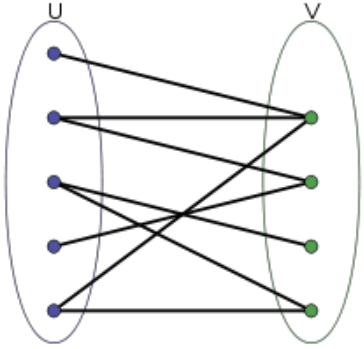
\includegraphics[width = 0.25\textwidth]{img/img9.png}
        \end{center}
    \end{definition}

    \begin{definition}[title = Matching]
        A matching in a graph is a subset of its edges such that no two edges have a node in common. \vspace{3.5pt}
        \begin{center}
            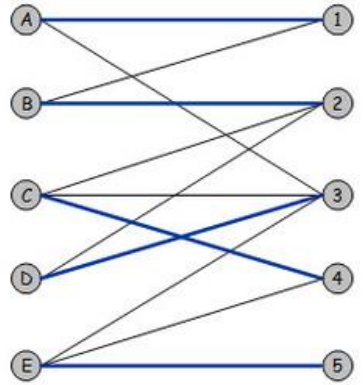
\includegraphics[width = 0.25\textwidth]{img/img10.png}
        \end{center} \vspace{3.5pt}
        \textbf{Maximal matching} is the largest possible matching. In a bipartite graph, maximal matching  covers one set of nodes.
    \end{definition}

    Therefore, combining together decision variables and their values we are able to determine if an assignment of those values is a solution or not.
    \begin{definition}[title = Solution]
        Given a \textbf{bipartite graph} $G$ constructed between the \textbf{variables} $[X_1, \dots, X_k]$ and their possible \textbf{values},
        an \textbf{assignment} of those values is a solution if and only if it corresponds to a \textbf{maximal matching} in $G$ (\textit{every couple of
        edges does not have a node in common}).
    \end{definition}
\end{itemize}
Generally, a bipartite graph is composed as in the image below. \vspace{3.5pt}
\begin{center}
    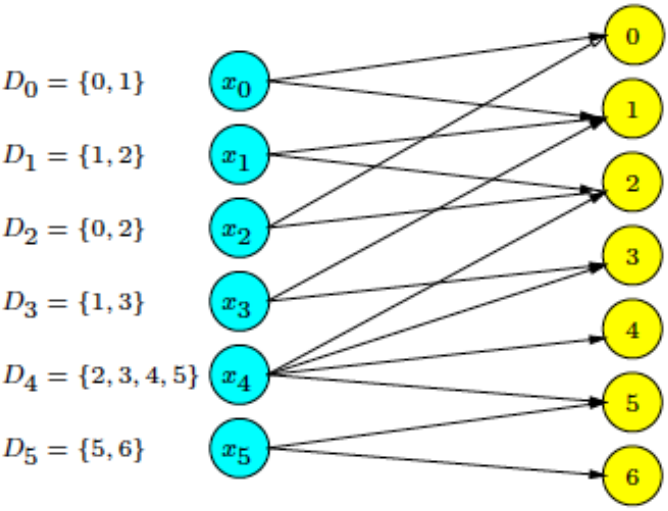
\includegraphics[width = 0.5\textwidth]{img/img11.png}
\end{center} \vspace{3.5pt}
The left side represents the set of all the decision variables with their respective domains, while in the right side we have all the different values. 
Every edge drawn in the previous representation defines a match between a decision variable and a value of its domain. A maximal matching is verified
when all the decision variables have a single no-shared match: a variable is linked to an one and only one value. \vspace{3.5pt}
\begin{center}
    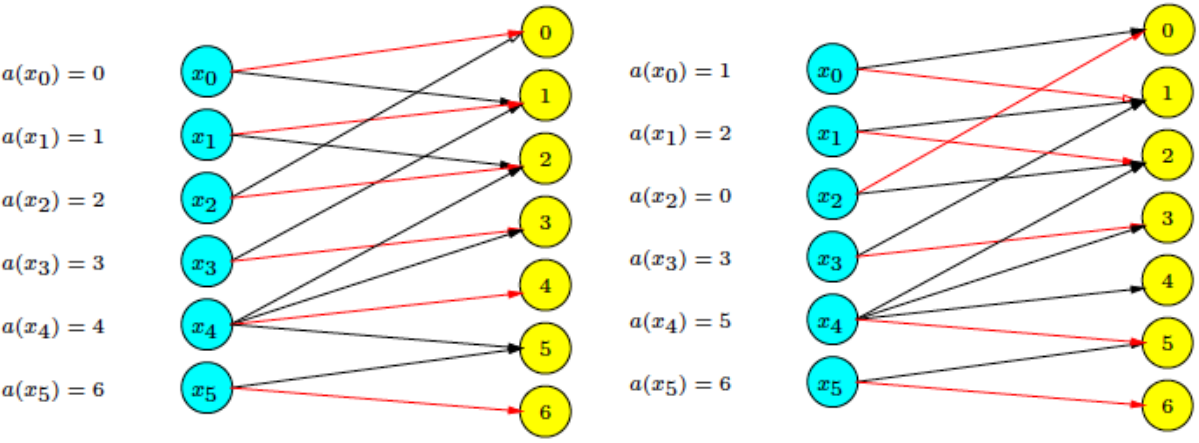
\includegraphics[width = 0.8\textwidth]{img/img12.png}
\end{center} \vspace{3.5pt}